\documentclass[30pt,landscape]{sciposter}

\usepackage{pstricks}
\usepackage[pdftex]{graphicx}
\usepackage{multirow,array}
\usepackage{amsmath,amsthm,amssymb}
\usepackage{algorithmic}
\usepackage{fancybox}
\usepackage{multicol}
\usepackage{natbib}

\definecolor{SectionCol}{rgb}{1.0,1.0,1.0}    %% section heading color
\definecolor{BoxCol}{rgb}{0.5,0.0,0.0}

\newtheorem*{theorem}{Theorem}
\newtheorem*{lemma}{Lemma}
\newtheorem*{definition}{Definition}
\newtheorem*{conjecture}{Conjecture}

\DeclareMathOperator*{\minimize}{minimize}
\DeclareMathOperator*{\Exp}{\mathbf{E}}
\DeclareMathOperator{\Regret}{Regret}
\DeclareMathOperator{\Reward}{Reward}
\DeclareMathOperator{\Wealth}{Wealth}
\DeclareMathOperator{\polylog}{polylog}
\DeclareMathOperator*{\argmin}{argmin}
\DeclareMathOperator*{\argmax}{argmax}

\newcommand{\R}{\mathbb{R}}
\renewcommand{\H}{\mathcal{H}}
\newcommand{\indicator}{\mathbf{1}}
\newcommand{\norm}[1]{\left\|#1\right\|}
\newcommand{\KL}[2]{\mathrm{KL}\left({#1} \, \middle\| \, {#2}\right)}
\newcommand{\grad}{\nabla}
\newcommand{\Breg}{\mathcal{B}}
\newcommand{\E}{\mathbb{E}}
\newcommand{\scO}{\mathcal{O}}

\begin{document}

\renewcommand{\thefootnote}{\fnsymbol{footnote}}
\renewcommand{\footlogo}{Typeset by pdf\LaTeX}
\renewcommand{\algorithmicrequire}{\textbf{Input:}}

\title{Coin Betting and Parameter-Free Online Learning}
\author{Francesco Orabona (Stony Brook University, NY), D\'avid P\'al (Yahoo Research, New York, NY)}

\date{December 5, 2016}

\leftlogo[1.2]{stony-brook-logo}
\rightlogo[1.2]{yahoo-logo}
\conference{The $30^{\text{th}}$ Annual Conference on Neural Information Processing Systems (NIPS), December 5--10, 2016, Barcelona, Spain}

\maketitle

\setlength{\parindent}{0em}
\setlength{\columnsep}{4cm}
\begin{multicols}{3}

\section*{Are you still tuning hyperparameters?}

Let $f$ a function convex in $w$.

Regularized empirical risk minimization:
$$
    \argmin_{w \in \R^d} \ \frac{\lambda}{2} \norm{w}^2 + \sum_{i=1}^T f(w, x_i, y_i)
$$
\begin{itemize}
\item How do you choose the regularizer weight $\lambda$?
\end{itemize}

\vspace{1cm}

Stochastic approximation:
$$
    w_t = w_{t-1} - \eta_t \widetilde{\grad} f(w_{t-1}, x_t, y_t)
$$
\begin{itemize}
\item How do you choose the learning rate $\eta_t$?
\end{itemize}

\vspace{1cm}

\begin{itemize}
\item Why is the algorithm not able to select $\lambda$ and/or $\eta_t$ automatically?
\end{itemize}

\section*{Online Learning and Coin Betting}

Let $V,V^*$ be a pair of dual vector spaces.

\vspace{1cm}

\setlength{\fboxrule}{5pt}
\setlength{\fboxsep}{10pt}
\begin{center}
Online Linear Optimization
\vspace{0.3cm}

\colorbox[rgb]{0.80,0.55,0.98}{\fbox{
\begin{minipage}{0.8\linewidth}
\begin{algorithmic}
{
\REQUIRE{Non-empty closed convex \emph{decision set} $K \subseteq V$}
\FOR{$t=1,2,3,\dots$}
\STATE Pick $w_t \in K$
\STATE Receive reward vector $g_t \in V^*$
\STATE Gain reward $\langle g_t, w_t \rangle$
\ENDFOR
}
\end{algorithmic}
\end{minipage}
}}
\end{center}

\vspace{0.5cm}

$$
\Regret_T(u) = \sum_{t=1}^T \langle g_t, u \rangle - \sum_{t=1}^T \langle g_t, w_t \rangle\; .
$$

\vspace{0.5cm}

\setlength{\fboxrule}{5pt}
\setlength{\fboxsep}{10pt}
\begin{center}
Coin Betting
\vspace{0.3cm}

\colorbox[rgb]{0.80,0.55,0.98}{\fbox{
\begin{minipage}{0.8\linewidth}
\begin{algorithmic}
{
\STATE $\Wealth_0 \leftarrow 1$
\FOR{$t=1,2,3,\dots$}
\STATE $\beta_t \leftarrow \frac{1}{t} \sum_{i=1}^{t-1} c_i$ \quad (KT estimator)
\STATE Bet $w_t = \beta_t \Wealth_{t-1}$
\STATE Observe coin flip $c_t \in \{+1, -1\}$
\STATE $\Wealth_t \leftarrow \Wealth_{t-1} \ + \ c_t \cdot w_t$
\ENDFOR
}
\end{algorithmic}
\end{minipage}
}}
\end{center}

Krichevsky-Trofimov showed that
$$
\Wealth_T \ge \exp\left( T \cdot \KL{\frac{1}{2} + \frac{\sum_{t=1}^T c_t}{2T} }{\frac{1}{2}} \right)
$$

\columnbreak

\section*{Parameter-Free Algorithms for Hilbert Spaces}

Let $\H$ be a Hilbert space. Let $K=\H$ and assume $\norm{g_t} \le 1$.
Gradient Ascent with learning rate $1/\sqrt{T}$ satisfies
$$
\forall u \in \H \qquad \Regret_T(u) \le \frac{1}{2}\left(1 + \norm{u}^2\right) \sqrt{T} \; .
$$
With learning rate $D/\sqrt{T}$, it satisfies
$$
\forall u : \norm{u} \le D  \qquad \Regret_T(u) \le D \sqrt{T} \; .
$$
Can we get
$$
\forall u \in \H \qquad \Regret_T(u) \le \norm{u} \sqrt{T} \; ?
$$

Addressed in Streeter\&McMahan (2012), Orabona (2013), McMahan\&Abernethy (2013), McMahan\&Orabona (2014), Orabona (2014).

But no intuition is given in previous contructions.

\vspace{1cm}

\begin{lemma}
Let $\Reward_T = \sum_{t=1}^T \langle g_t, w_t \rangle$.
Let $F:K \to \R$ be convex.
$$
\big( \forall u \in K \quad \Regret_T(u) \le F(u) \big)
\quad \text{if and only if} \quad
\Reward_T \ge F^*\left(\sum_{t=1}^T g_t\right) \; .
$$
\end{lemma}



\vspace{0.5cm}

\setlength{\fboxrule}{5pt}
\setlength{\fboxsep}{10pt}
\begin{center}
Coin Betting for Hilbert Spaces
\vspace{0.3cm}

\colorbox[rgb]{0.80,0.55,0.98}{\fbox{
\begin{minipage}{0.8\linewidth}
\begin{algorithmic}
{
\STATE $L_0 \leftarrow 0$
\STATE $\Wealth_0 \leftarrow 1$
\FOR{$t=1,2,3,\dots$}
\STATE Predict $w_t = \frac{\Wealth_{t-1}}{t} \,  G_{t-1}$
\STATE Observe $g_t \in \H$ such that $\norm{g_t} \le 1$
\STATE $G_t \leftarrow G_{t-1} + g_t$
\STATE $\Wealth_t \leftarrow \Wealth_{t-1} \ + \ \langle g_t, w_t \rangle$
\ENDFOR
}
\end{algorithmic}
\end{minipage}
}}
\end{center}

Generalizing Krichevsky-Trofimov,
$$
1 + \Reward_T = \Wealth_T \ge \exp\left( T \cdot \KL{\frac{1}{2} + \frac{\norm{\sum_{t=1}^T g_t}}{2T} }{\frac{1}{2}} \right)
$$
Using the Lemma, we get $\Regret_T(u) \le \norm{u} \sqrt{T \ln(1 + 24 T^2 \norm{u}^2)} + 1$.

\vspace{0.5cm}

Setting $g_t=\widetilde{\grad} f(w_t,x_t,y_t)$ and online-to-batch conversion gives in expectation
$$
\E_{x,y} \left[f\left(\hat{w}, x,y\right)\right]
\leq \scO\left(\min_{u} \min_{\lambda>0} \ \E_{x,y}\left[f\left(u, x, y\right)\right] + \lambda \norm{u}^2 +\frac{\ln(T)}{\lambda \, T} \right)
$$



\columnbreak

\section*{Parameter-Free Algorithms for Learning with Expert Advice}

Let $K=\Delta_N$ and assume $g_t \in [0,1]^N$.
Hedge with learning rate $\eta$ satisfies
\[
\forall u \in \Delta_N \qquad
\Regret_T(u) \leq O \left(\tfrac{\KL{u}{\pi}}{\eta} + \eta T \right)
\]
With learning rate $\eta = D/\sqrt{T}$, it satisfies
$$
\forall u : \KL{u}{\pi} \le D  \qquad \Regret_T(u) \le \sqrt{T \cdot D} \; .
$$
Can we get
$$
\forall u \in \Delta_N \qquad \Regret_T(u) \le \sqrt{T \cdot \KL{u}{\pi}} \; ?
$$

Addressed in Chaudhuri et al. (2009), Chernov\&Vovk (2010), Luo\&Schapire (2014, 2015), Koolen\&van-Erven (2015), Foster et al. (2015).
But no intuition is given in previous contructions.

\vspace{1cm}

\begin{center}
Learning with Expert Advice
\vspace{0.3cm}

\colorbox[rgb]{0.80,0.55,0.98}{\fbox{
\begin{minipage}{0.8\linewidth}
\begin{algorithmic}
{
\REQUIRE{\#experts $N$, prior $\pi \in \Delta_N$, \#rounds $T$}
\FOR{$t=1,2,\dots,T$}
\STATE{For each $i \in [N]$, set $w_{t,i} \leftarrow \tfrac{\sum_{j=1}^{t-1} \widetilde g_{j,i}}{t+T/2} \left(1 + \sum_{j=1}^{t-1} \widetilde g_{j,i} w_{j,i} \right)$}
\STATE{For each $i \in [N]$, set $\widehat{p}_{t,i} \leftarrow \pi_i [w_{t,i}]_+$}
\STATE{Predict with $p_t \leftarrow
\begin{cases}
\widehat{p}_t/\norm{\widehat{p_t}}_1 & \text{if $\norm{\widehat p_t}_1 > 0$} \\
\pi & \text{if $\norm{\widehat p_t}_1 = 0$}
\end{cases}$}
\STATE{Receive reward vector $g_t \in [0,1]^N$}
\STATE{For each $i \in [N]$, set $\widetilde g_{t,i} \leftarrow \begin{cases}
g_{t,i} - \langle g_t, p_t \rangle & \text{if $w_{t,i} > 0$} \\
[g_{t,i} - \langle g_t, p_t \rangle]_+ & \text{if $w_{t,i} \le 0$}
\end{cases}$}
\ENDFOR
}
\end{algorithmic}
\end{minipage}
}}
\end{center}

\vspace{1cm}

\begin{theorem}
The algorithm
for any $g_1, g_2, \dots, g_T \in [0,1]^N$ satisfies
\[
\forall u \in \Delta_N \qquad \qquad \Regret_T(u) \le \sqrt{3T (3 + \KL{u}{\pi})} \; .
\]
\end{theorem}

\section*{Empirical Evaluation}

\centering{
\begin{tabular}{ccc}
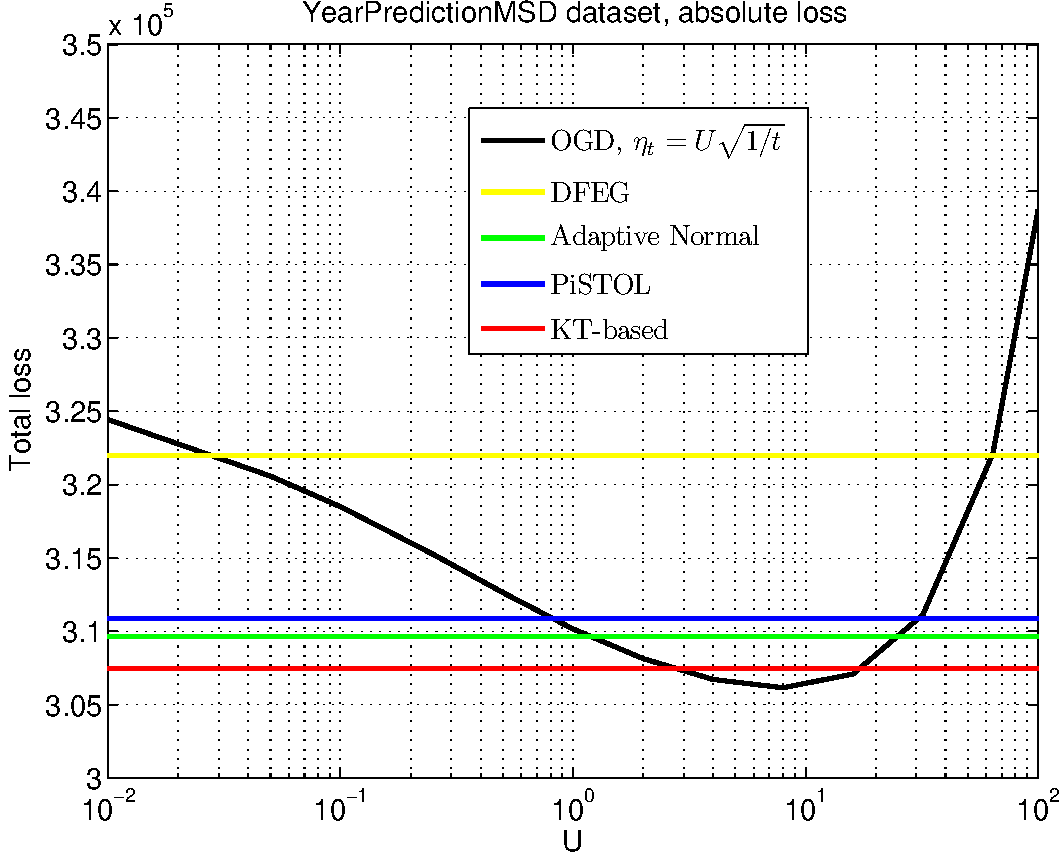
\includegraphics[width=0.30\linewidth]{../NIPS-2016-camera-ready/figs/yearpredictionmsd_kt-crop.pdf} &
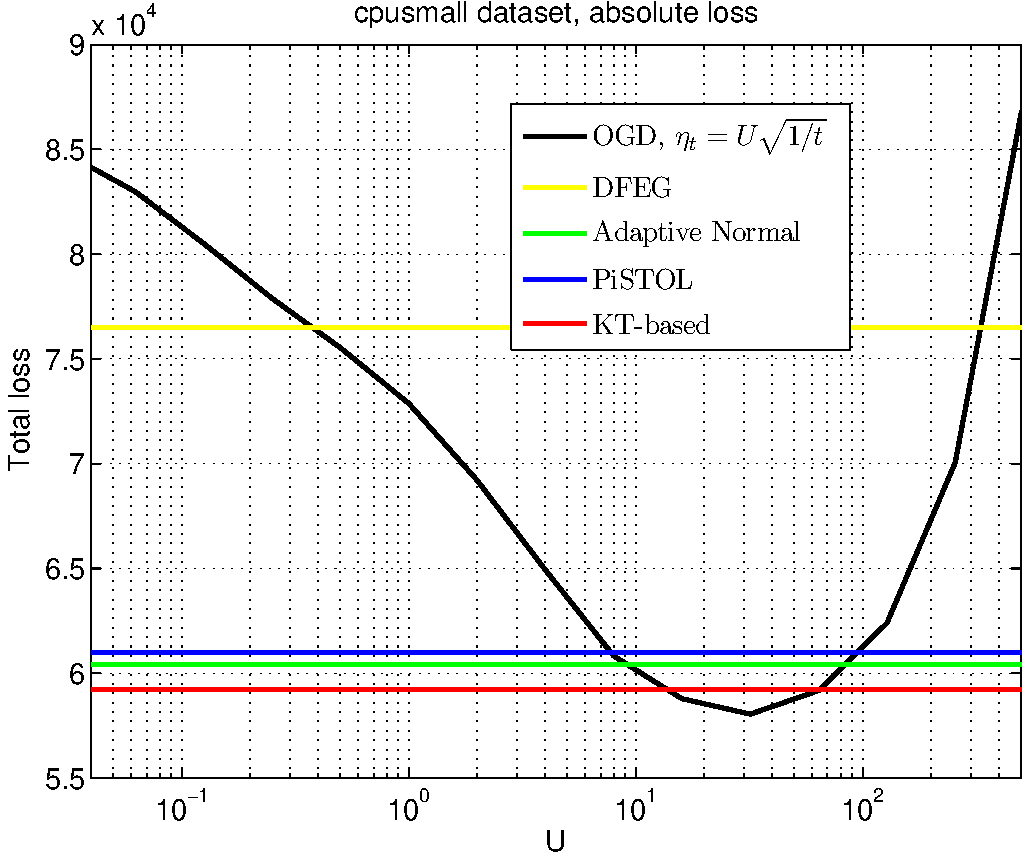
\includegraphics[width=0.30\linewidth]{../NIPS-2016-camera-ready/figs/cpusmall_kt-crop.pdf} &
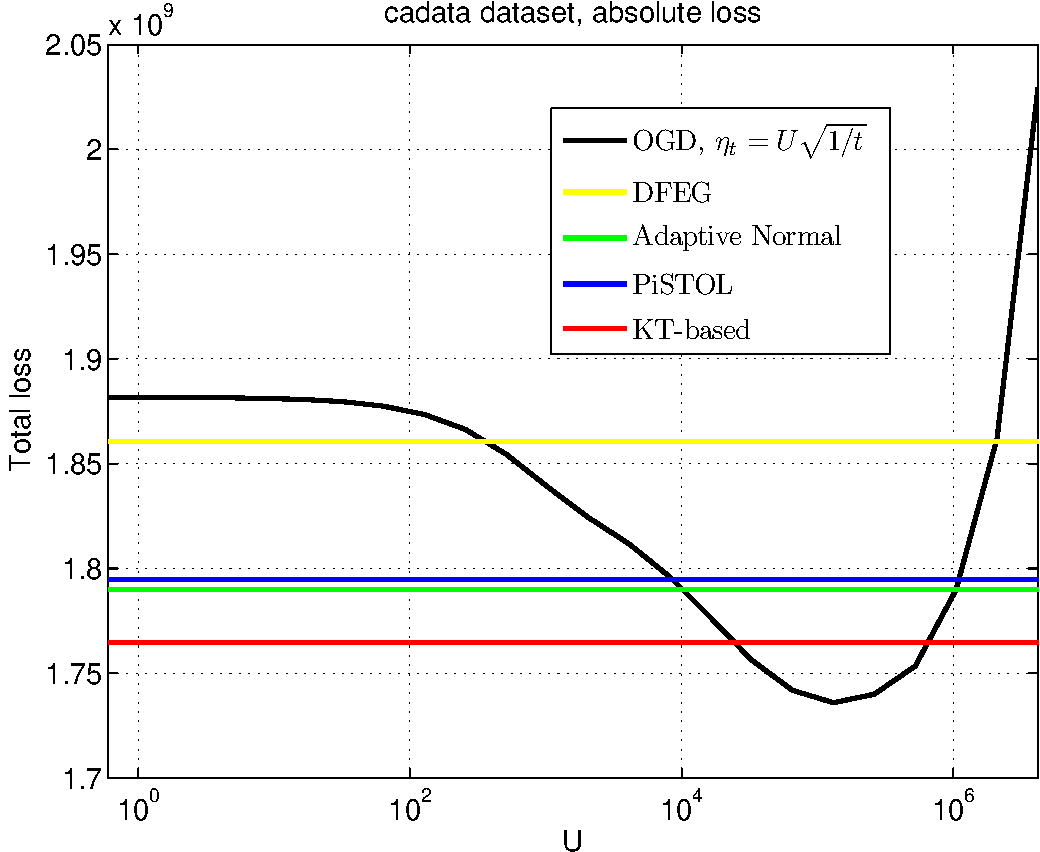
\includegraphics[width=0.30\linewidth]{../NIPS-2016-camera-ready/figs/cadata_kt-crop.pdf}
\end{tabular}

\footnotesize{Total loss versus learning rate parameter of OGD, compared with parameter-free algorithms.}

\begin{tabular}{ccc}
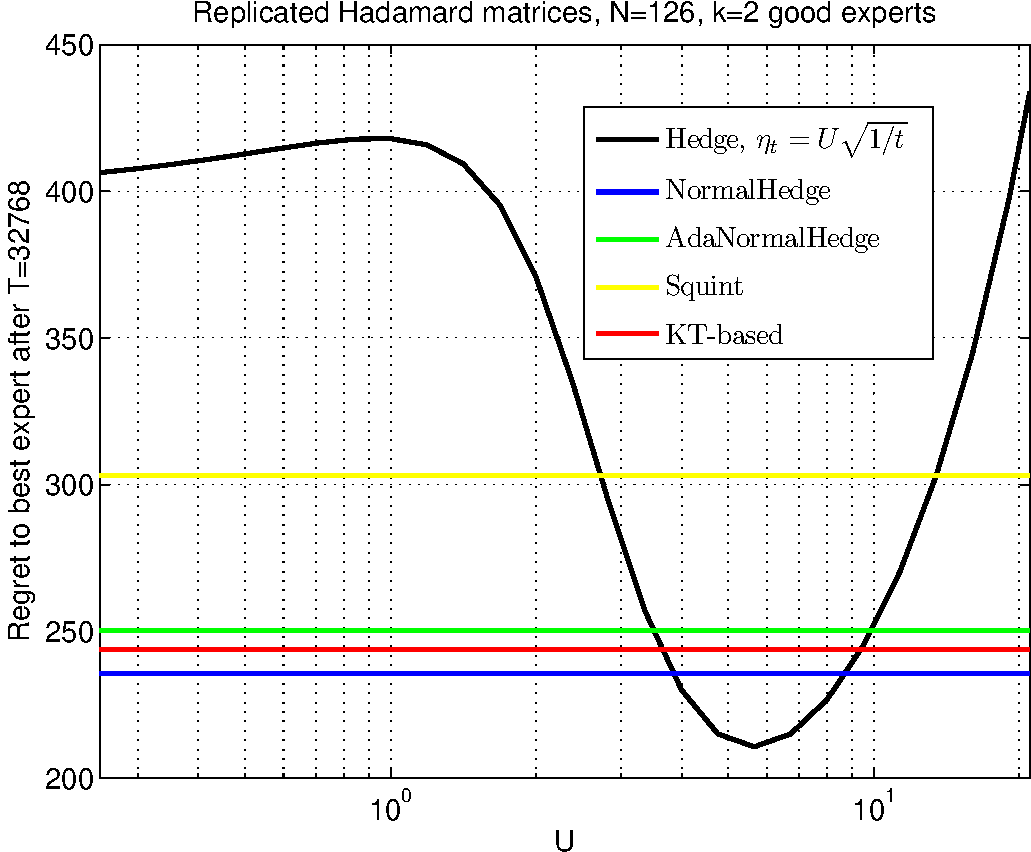
\includegraphics[width=0.30\linewidth]{../NIPS-2016-camera-ready/figs/fig1-crop.pdf} &
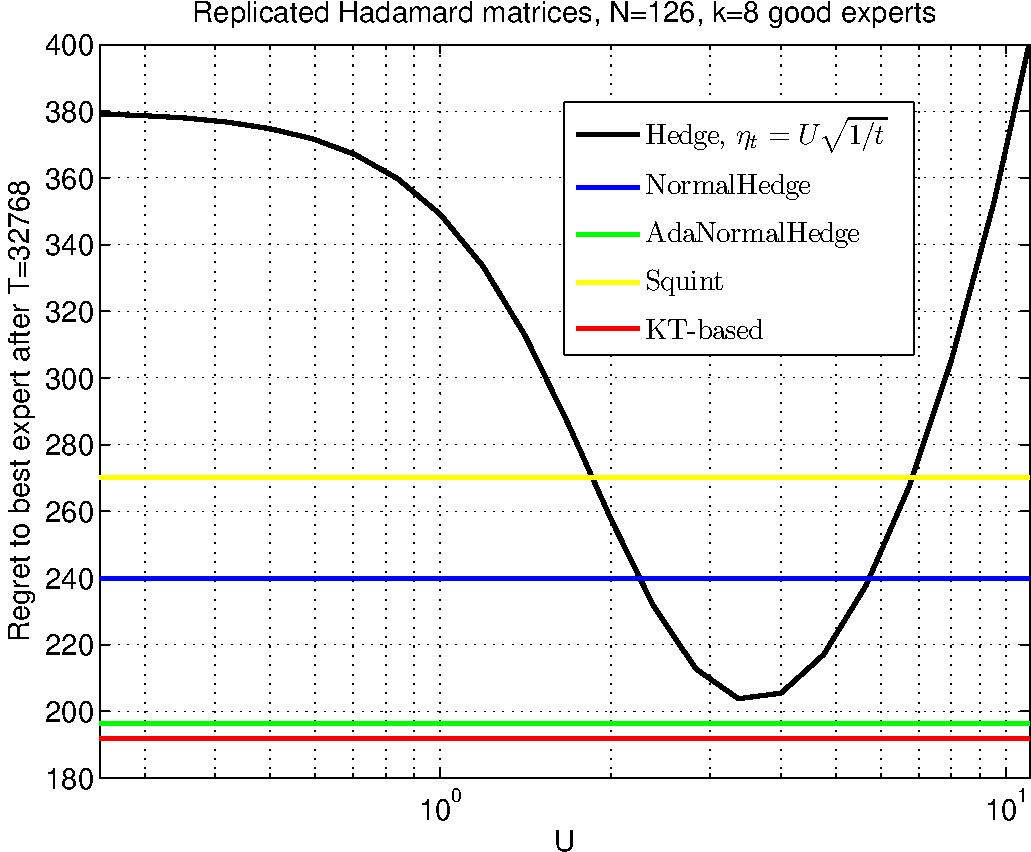
\includegraphics[width=0.30\linewidth]{../NIPS-2016-camera-ready/figs/fig2-crop.pdf} & 
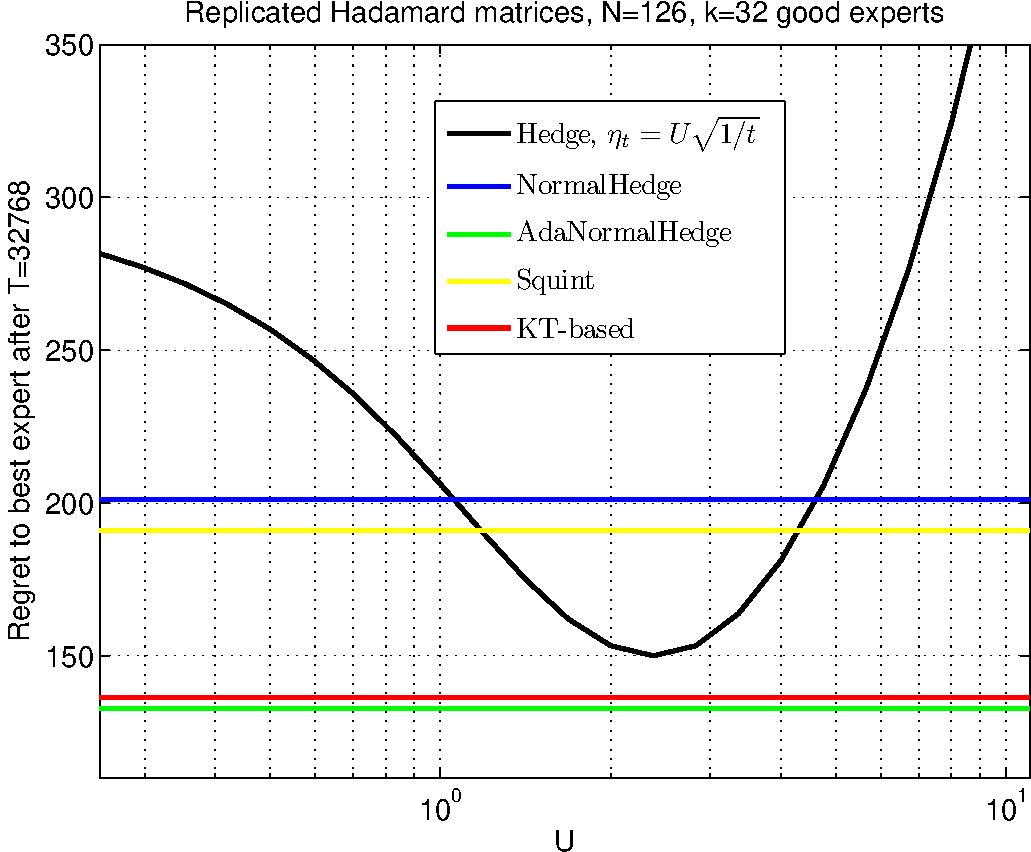
\includegraphics[width=0.30\linewidth]{../NIPS-2016-camera-ready/figs/fig3-crop.pdf}
\end{tabular}

\footnotesize{Regrets to the best expert after $T = 32768$ rounds,
versus learning rate parameter of Hedge. The ``good'' experts
are $\epsilon=0.025$ better than the others. $\pi_i=1/N$ for all
algorithms.}
}
\end{multicols}

\end{document}
